%%%%%%%%%%%%%%%%%%%%%%%%%%%%%%%%%%%%%%%%%
% Beamer Presentation
% LaTeX Template
% Version 1.0 (10/11/12)
%
% This template has been downloaded from:
% http://www.LaTeXTemplates.com
%
% License:
% CC BY-NC-SA 3.0 (http://creativecommons.org/licenses/by-nc-sa/3.0/)
%
%%%%%%%%%%%%%%%%%%%%%%%%%%%%%%%%%%%%%%%%%


%------------------------------------------------------u h tb t  ----------------------------------
%	PACKAGES AND THEMES
%----------------------------------------------------------------------------------------

\documentclass{beamer}

\mode<presentation> 

\usepackage{xcolor}
\usepackage{graphicx}
\usepackage{subcaption}
\usepackage{tikz}



\setbeamertemplate{itemize items}[default]
\setbeamertemplate{enumerate items}[default]
% The Beamer class comes with a number of default slide themes
% of all the themes, uncomment each in turn to see what they look like.

%\usetheme{default}
% \usetheme{AnnArbor}
% \usetheme{Antibes}
% \usetheme{Bergen}
%\usetheme{Berkeley}
% \usetheme{Berlin}
% \usetheme{Boadilla}
\usetheme{CambridgeUS}
% \usetheme{Copenhagen}
%\usetheme{Darmstadt}
%\usetheme{Dresden}
% \usetheme{Frankfurt}
%\usetheme{Goettingen}
%\usetheme{Hannover}
% \usetheme{Ilmenau}
% \usetheme{JuanLesPins}
%\usetheme{Luebeck}
%\usetheme{Madrid}
%\usetheme{Malmoe}
%\usetheme{Marburg}
%\usetheme{Montpellier}
% \usetheme{PaloAlto}
%\usetheme{Pittsburgh}
%\usetheme{Rochester}
% \usetheme{Singapore}
%\usetheme{Szeged}
%\usetheme{Warsaw}

% As well as themes, the Beamer class has a number of color themes
% for any slide theme. Uncomment each of these in turn to see how it
% changes the colors of your current slide theme.

%\usecolortheme{albatross}
% \usecolortheme{beaver}
% \usecolortheme{beetle}
% \usecolortheme{crane}
\usecolortheme{dolphin}
% \usecolortheme{dove}
% \usecolortheme{fly}
% \usecolortheme{lily}
% \usecolortheme{orchid}
%\usecolortheme{rose}
%\usecolortheme{seagull}
% \usecolortheme{seahorse}
%\usecolortheme{whale}
%\usecolortheme{wolverine}

%\setbeamertemplate{footline} % To remove the footer line in all slides uncomment this line
%\setbeamertemplate{footline}[page number] % To replace the footer line in all slides with a simple slide count uncomment this line

%\setbeamertemplate{navigation symbols}{} % To remove the navigation symbols from the bottom of all slides uncomment this line

\setbeamertemplate{blocks}[shadow=false]
% \setbeamercolor{block title}{bg=cyan, fg=white}
% \setbeamercolor{block body}{bg=cyan!10}



\usepackage{graphicx} % Allows including images
\usepackage{booktabs} % Allows the use of \toprule, \midrule and \bottomrule in tables
\usepackage{xcolor}
\setcounter{tocdepth}{1}


%----------------------------------------------------------------------------------------
%	TITLE PAGE
%----------------------------------------------------------------------------------------

\title[Oral Qualification Examination]{Unbiased Stochastic Gradient Descent for Strongly Correlated Time Series Data} % The short title appears at the bottom of every slide, the full title is only on the title page

\author{Unknown} % Your name
\institute[IORA] % Your institution as it will appear on the bottom of every slide, may be shorthand to save space
{
Supervisor: Unknown\\
National University of Singapore \\ % Your institution for the title page


\medskip
%\textit{john@smith.com} % Your email address
}
\date{\today} % Date, can be changed to a custom date

\begin{document}





\begin{frame}
\titlepage % Print the title page as the first slide
\end{frame}






\begin{frame}
\frametitle{Outline} % Table of contents slide, comment this block out to remove it
\tableofcontents % Throughout your presentation, if you choose to use \section{} and \subsection{} commands, these will automatically be printed on this slide as an overview of your presentation
\end{frame}

%----------------------------------------------------------------------------------------
%	PRESENTATION SLIDES

\section{Formal optimization problem}
\begin{frame}{Formal optimization problem}
    \begin{itemize}
        \item Quantity of interest: $y_t = y(w^*,x_t,\xi_t)$
        \item Parameterized prediction of $y_t$: $\hat{y}_t=\hat{y}(w,x_t)$
        \item 
        Expected loss function to quantify the error: $F(w) = E_{X,Y}[f(w,X,Y)]$
        \item Optimization objective: find $w^*=\underset{w}{argmin}\:F(w)$
        
    \end{itemize}

    \begin{tikzpicture}[overlay, remember picture]
        % Define nodes at specific coordinates relative to the current page
        \node (target1) at (4.3, 1.9) {};
        \node (target2) at (4.5, 1.9) {};
        \node (target3) at (4.9, 1.9) {};
        \node (source1) at (2.3, 3.5) {};
        \node (source2) at (5.8, 3.5) {};
        \node (source3) at (6.9, 3.5) {};

        % Draw arrows pointing to the targets
        %\draw[->, black, thick] (source1) -- (target1) node[midway, above, sloped] {Data};
        %\draw[->, black, thick] (source2) -- (target2) node[midway, above, sloped] {Parameters};
        %\draw[->, black, thick] (source3) -- (target3) node[midway, above, sloped] {Noise};
    \end{tikzpicture}

    
\end{frame}

\section{Vanilla SGD}
\begin{frame}{Vanilla SGD}
\begin{itemize}
    \item Costly using gradient descent: $w_{t+1}=w_t-\eta_{t+1}\nabla_w F(w_t)$\\
    \item Idea: Use sample estimation of $\nabla_w F(w_t)$ as $\nabla_w f(w_t,x_{t+1},y_{t+1})$
    \\$\;\;\;\;\;\;\;\;\;\rightarrow$ SGD: $w_{t+1}=w_t-\eta_{t+1}\nabla_w f(w_t,x_{t+1},y_{t+1})$
    \item \textcolor{red}{Key assumption}: ($X_t$,$Y_t$) are \textcolor{red}{i.i.d}, hence by LLN
    \begin{equation*}
        E_t[\nabla_w f(w,x_{t+1},y_{t+1})]=\nabla_w F(w)
    \end{equation*}
\end{itemize}
\end{frame}

\section{Problem with correlated data}
\begin{frame}{Problem with correlated data}
    \begin{itemize}
        \item We consider the setting when the x-data is generated by a stationary AR(1) process
        \item Normal for financial data such as portfolio returns
        \item Hence $X_t$-data are auto-correlated, and ($X_t$,$Y_t$) are no longer i.i.d.
        \item Sample gradient biased: $E_t[\nabla_w f(w,x_{t+1},y_{t+1})]\neq \nabla_w F(w)$
        \item For highly correlated data, standard SGD will suffer significantly
    \end{itemize}
\end{frame}

\section{Unbiased SGD - Main Idea}
\begin{frame}{Main idea - Unbiased SGD}
    \begin{itemize}
        \item Find $Q_t$ such that:\\
        \begin{equation*}
            Q_tE_t[\nabla_w f(w,x_{t+1},y_{t+1})] = \nabla_w F(w)
        \end{equation*}
        \item Perform the following \textcolor{red}{unbiased} SGD updates:\\
        \begin{equation*}
            w_{t+1} = w_t - \eta_{t+1}\textcolor{red}{Q_t}\nabla_w f(w_t,x_{t+1},y_{t+1})
        \end{equation*}
    \end{itemize}
\end{frame}

\section{Linear Univariate Case}
\begin{frame}{Linear Univariate Case - Model}
Data generating process:
\begin{itemize}
    \item $x$-data: $x_{t+1} = \rho x_t + \epsilon_{t+1}$, \;\;$\rho<1$ {\hfill \textit{AR(1)}}
    \item $y$-data: $y_{t+1}=w^*x_{t+1} + \xi_{t+1}$ {\hfill \textit{Linear regression model}}
\end{itemize}
Prediction:
\begin{itemize}
    \item $\hat{y}_{t+1} = wx_{t+1}${\hfill \textit{Linear regression estimate}}
\end{itemize}
Loss function:
\begin{itemize}
    \item $f(w,x,y)=\frac{1}{2}(wx-y)^2$ \hfill\textit{$L_2$-loss}
\end{itemize}
\end{frame}

\begin{frame}{Linear Univariate Case - Finding $Q_t$}
    \begin{itemize}
        \item Want to find $Q_t$ such that: $Q_tE_t[\nabla_w f(w,X_{t+1},Y_{t+1})]=E[\nabla_w f(w,X_{t+1},Y_{t+1})]$
        \newline
        \item Can calculate:
        \begin{itemize}
            \item $E_t[\nabla_w f(w,X_{t+1},Y_{t+1})]=[\rho^2x_t^2+\sigma_\epsilon^2](w-w^*)$
            \item $E[\nabla_w f(w,X_{t+1},Y_{t+1})]=\sigma_x^2(w-w^*)$
            \newline
        \end{itemize}
        \item $Q_t$ given as:\\
        \begin{equation*}
            Q_t = \frac{\sigma_x^2}{\rho^2x_t^2+\sigma_\epsilon^2}
        \end{equation*}
    \end{itemize}
\end{frame}

\begin{frame}{Linear Univariate Case - Intuition of $Q_t$}
For stationary AR(1) process, $\sigma_\epsilon^2=(1-\rho^2)\sigma_x^2$:
\begin{equation*}
    Q_t = \frac{\sigma_x^2}{\sigma_x^2 + \textcolor{red}{\rho^2(x_t^2-\sigma_x^2)}}
\end{equation*}

Hence,
\begin{equation*}
    Q_t=\begin{cases}
        &>1, \quad if\; x_t^2<\sigma_x^2\\
        &=1, \quad if\; x_t^2=\sigma_x^2\\
        &<1, \quad if\; x_t^2>\sigma_x^2\\
    \end{cases}
\end{equation*}

While the conditionally expected error is given as

\begin{equation*}
    E_t[error_{t+1}]=E_t[\hat{y}_{t+1}-y_{t+1}]=\rho x_t(w_t-w^*)
\end{equation*}

    
\end{frame}

\begin{frame}{Linear Univariate Case - Results}
    Convergence to $E[(w_{t+1}-w^*)^2]\leq\Delta$:\\
    \begin{columns}
        \begin{column}{0.483\textwidth}
            \newline 
            \textbf{Vanilla SGD:}
            \begin{itemize}
                \item  $t \geq \Omega\left(\frac{log(\Delta)}{\Delta \textcolor{red}{(1-\rho^2)^2}}\right) $
            \end{itemize}
        \end{column}
        \begin{column}{0.483\textwidth}
            \newline 
            \textbf{Unbiased SGD:}
            \begin{itemize}
                \item $t \geq \Omega\left(\frac{log(\Delta)}{\Delta\textcolor{red}{ (1-\rho^2)}}\right)$
            \end{itemize}
        \end{column}
    \end{columns}
    \textbf{Numerical:}
    \begin{figure}[h]
    \centering
    \begin{subfigure}{0.45\textwidth}
        \centering
        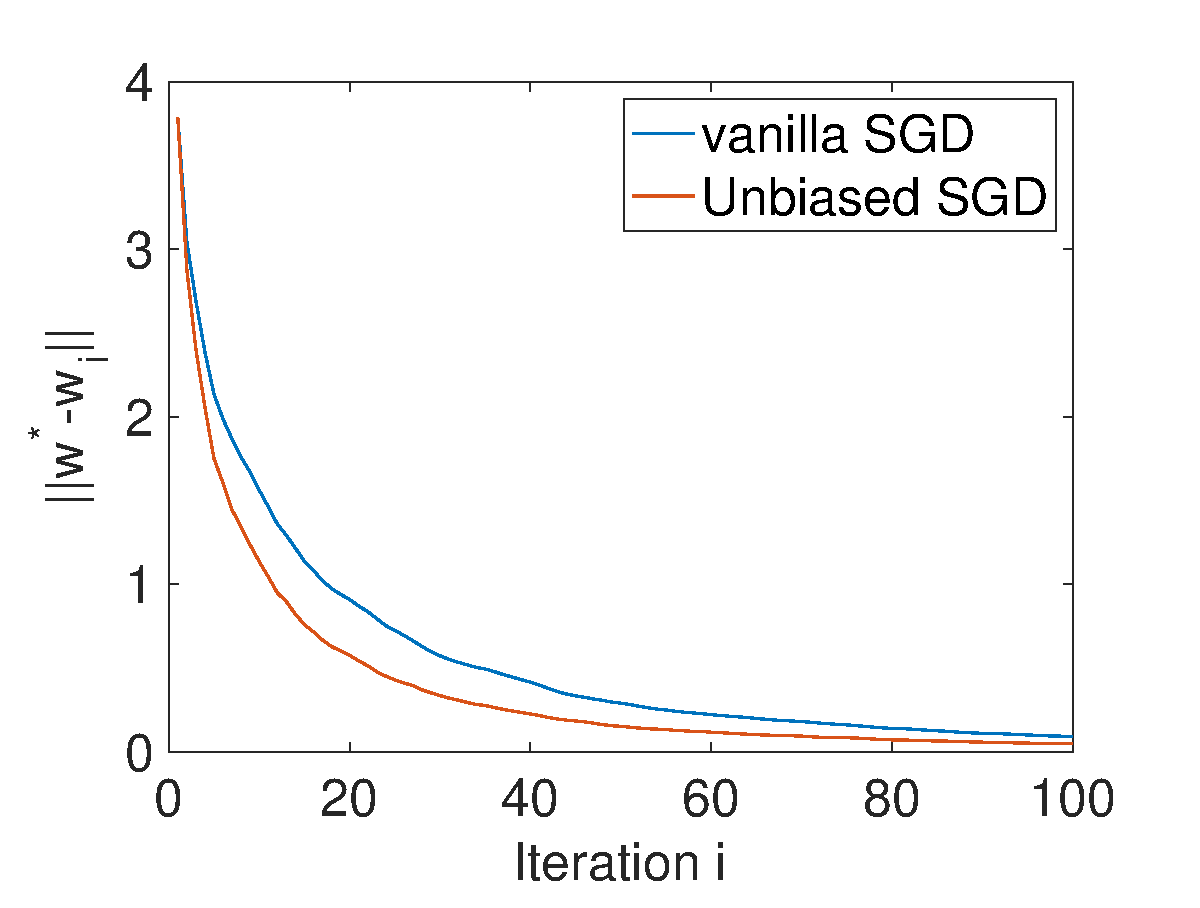
\includegraphics[width=\textwidth]{AR1_rho08.eps}
        \caption{$\rho=0.8$}
        \label{fig:image1}
    \end{subfigure}
    \hfill
    \begin{subfigure}{0.45\textwidth}
        \centering
        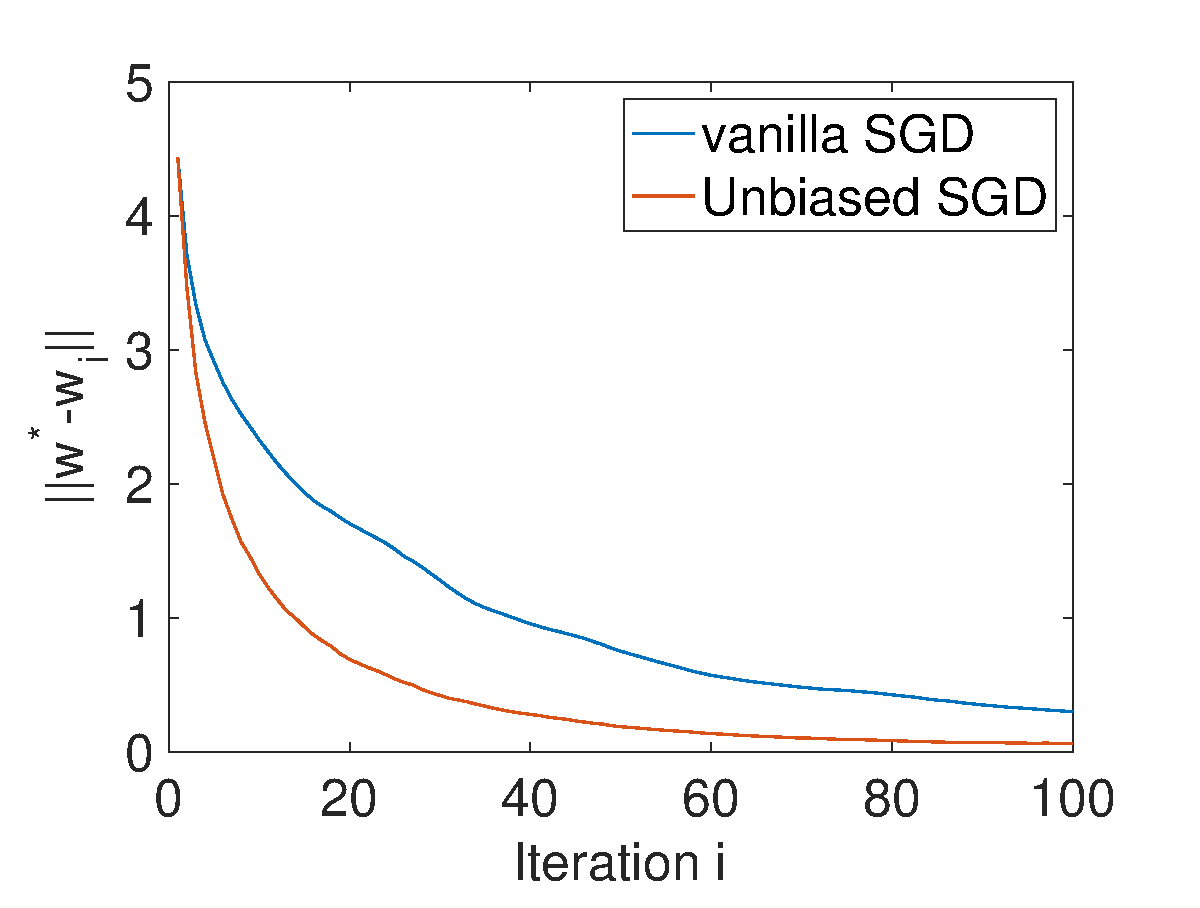
\includegraphics[width=\textwidth]{AR1_rho095.eps}
        \caption{$\rho=0.95$}
        \label{fig:image2}
    \end{subfigure}
    %\caption{A figure with two subfigures}
    \label{fig:side_by_side}
\end{figure}
\end{frame}


\section{Linear Multivariate Case}
\begin{frame}{Linear Multivariate Case - Model}
Data generating process:
\begin{itemize}
    \item $x$-data: $x_{t+1} = P x_t + \epsilon_{t+1}$, \;\;$\lambda_{max}(P)<1$ {\hfill \textit{AR(1)}}
    \item $y$-data: $y_{t+1}=x_{t+1}^Tw^* + \xi_{t+1}$ {\hfill \textit{Linear regression model}}
\end{itemize}
Prediction:
\begin{itemize}
    \item $\hat{y}_{t+1} = x_{t+1}^Tw${\hfill \textit{Linear regression estimate}}
\end{itemize}
Loss function:
\begin{itemize}
    \item $f(w,x,y)=\frac{1}{2}(x^Tw-y)^2$ \hfill\textit{$L_2$-loss}
\end{itemize}
    
\end{frame}

\begin{frame}{Linear Multivariate Case - Finding $Q_t$}
    \begin{itemize}
        \item Want to find $Q_t$ such that: $Q_tE_t[\nabla_w f(w,X_{t+1},Y_{t+1})]=E[\nabla_w f(w,X_{t+1},Y_{t+1})]$
        \newline
        \item Can calculate:
        \begin{itemize}
            \item $E_t[\nabla_w f(w,X_{t+1},Y_{t+1})]=[Px_tx_t^TP^T+\Sigma_\epsilon](w-w^*)$
            \item $E[\nabla_w f(w,X_{t+1},Y_{t+1})]=\Sigma_x(w-w^*)$
            \newline
        \end{itemize}
        \item $Q_t$ given as:\\
        \begin{equation*}
            Q_t = \Sigma_x[Px_tx_t^TP^T+\Sigma_\epsilon]^{-1}
        \end{equation*}
    \end{itemize}
\end{frame}

\begin{frame}{Linear Multivariate Case - Results}
    Convergence to $E[||w_{t+1}-w^*||^2]\leq\Delta$:\\
    \newline
    \begin{columns}
        \begin{column}{0.483\textwidth}
            \newline 
            \textbf{Vanilla SGD:}
            \begin{itemize}
                \item  $t \geq \Omega\left(\frac{log(\Delta)}{\Delta \textcolor{red}{(\lambda_{\epsilon}^{min})^2}}\right)$
            \end{itemize}
        \end{column}
        \begin{column}{0.483\textwidth}
            \newline 
            \textbf{Unbiased SGD:}
            \begin{itemize}
                \item $t \geq \Omega\left(\frac{log(\Delta)}{\Delta\textcolor{red}{ \lambda_{\epsilon}^{min}}}\right)$
            \end{itemize}
        \end{column}
    \end{columns}\\
    Note: $\Sigma_\epsilon = \Sigma_x-P\Sigma_xP^T\rightarrow 0$ as $\lambda_P^{min}\rightarrow1$\\
    \textbf{Numerical:}
    \begin{figure}[h]
    \centering
    \begin{subfigure}{0.45\textwidth}
        \centering
        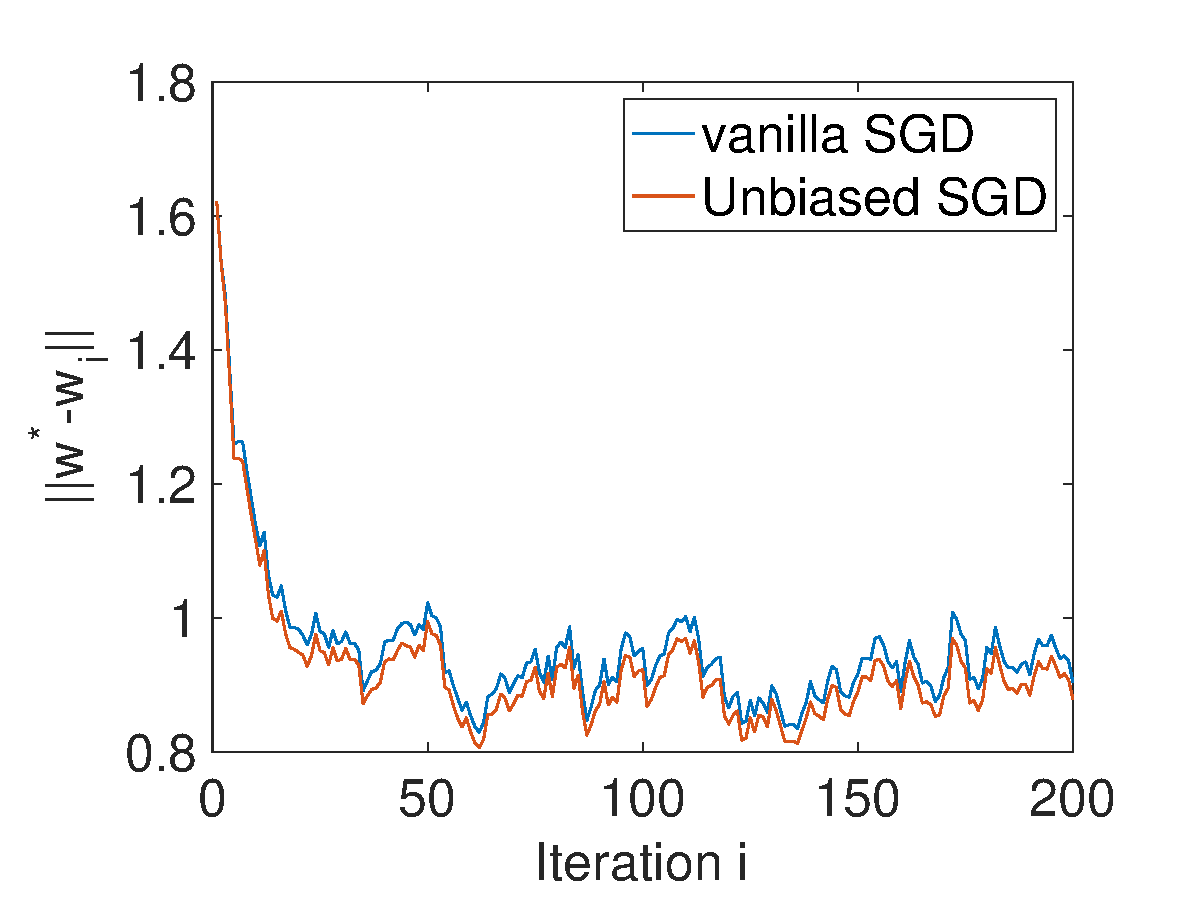
\includegraphics[width=\textwidth]{AR1_rho01Multivariate.eps}
        \caption{$\lambda_P^{min}=0.1$}
        \label{fig:image1}
    \end{subfigure}
    \hfill
    \begin{subfigure}{0.45\textwidth}
        \centering
        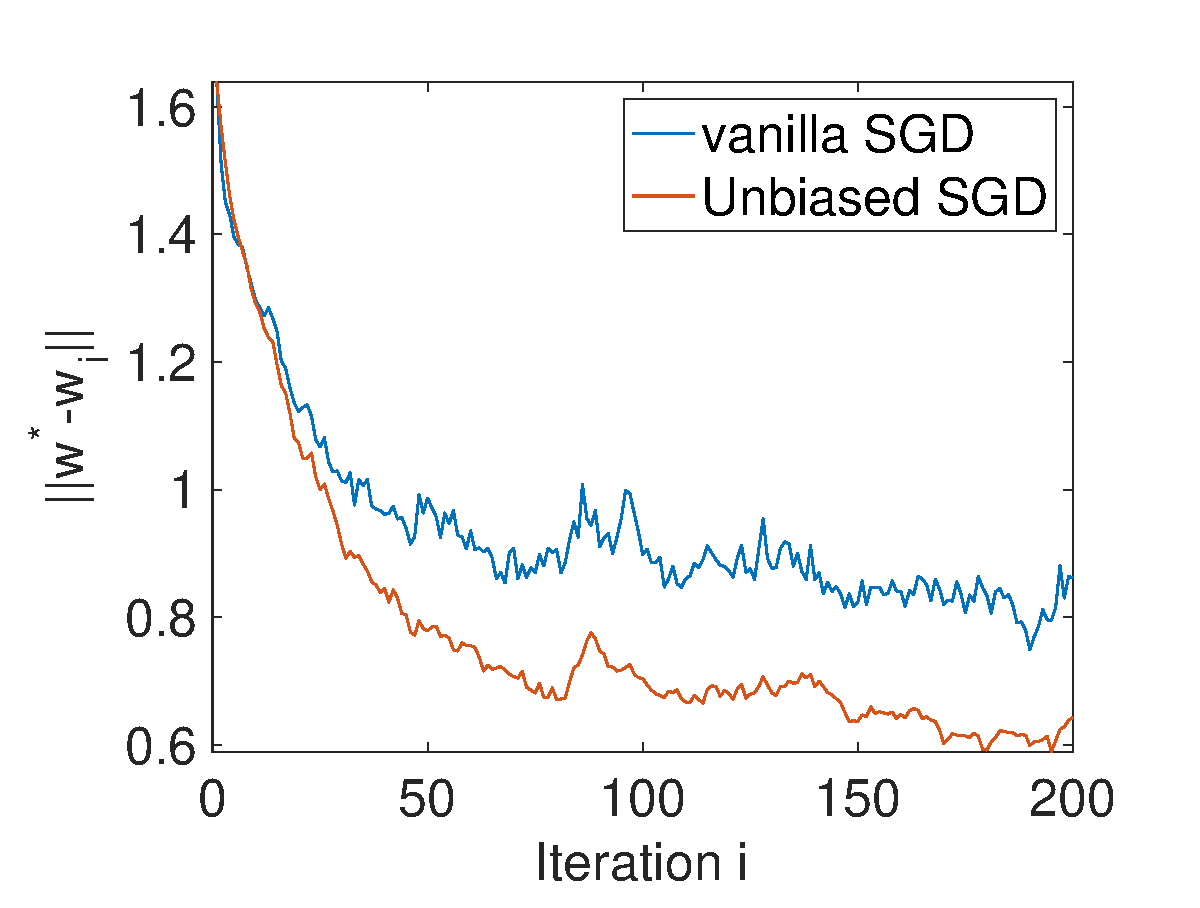
\includegraphics[width=\textwidth]{AR1_rho09Multivariate.eps}
        \caption{$\lambda_P^{min}=0.9$}
        \label{fig:image2}
    \end{subfigure}
    \vspace{-10pt}
    %\caption{Correlation matrix $P=\rho I$, $\Sigma_\epsilon = \Sigma_x - P\Sigma_xP^T$}
    \label{fig:side_by_side}
\end{figure}
\end{frame}

\section{General Unbiased SGD}
\begin{frame}{General Unbiased SGD - Generalizing further}
    \begin{itemize}
        \item Want to consider more general class of functions $f$
        \item Conditions:
        \begin{itemize}
            \item $\nabla_w f(w,x,y)$ and $H_f(w,x,y)$ known
            \item $E_t[\nabla_w f(\textcolor{red}{w^*},X_{t+1},Y_{t+1})]=E[\nabla f(\textcolor{red}{w^*},X_{t+1},Y_{t+1})]=0$
        \end{itemize}
    \end{itemize}
\end{frame}

\begin{frame}{General Unbiased SGD - Finding $Q_t$}
How to find $Q_t$ such that:
\begin{equation*}
    Q_tE_t[\nabla_wf(\bm{w}_{t},X_{t+1},Y_{t+1})] = E[\nabla_wf(\bm{w},X_{t+1},Y_{t+1})]
\end{equation*}
    \textbf{Main idea:}\\
    If
    \begin{equation*}
    \begin{cases}
&Q_tE_t[\nabla_wf(\bm{w}_{t},X_{t+1},Y_{t+1})] \approx Q_t\bm{A}\bm{c} \\
&E[\nabla_wf(\bm{w},X_{t+1},Y_{t+1})] \approx \bm{B}\bm{c}
    \end{cases}
\end{equation*}
then 
\begin{equation*}
    \bm{Q_t} \approx \bm{A}^{-1}\bm{B}.
\end{equation*} 
\end{frame}

\begin{frame}{General Unbiased SGD - Calculating $Q_t$}
    Taylor expansion around $w^*$:
    \begin{equation*}
    \nabla_w f(\bm{w},X_{t+1},Y_{t+1}) \approx \nabla_w f(\bm{w}^*,X_{t+1},Y_{t+1}) + H_{f_w}(\bm{w}^*,X_{t+1},Y_{t+1}) (\bm{w}^*-\bm{w}).
\end{equation*}
By
\begin{equation*}
    E_t[\nabla_w f(w^*,X_{t+1},Y_{t+1})]=E[\nabla_w f(w^*,X_{t+1},Y_{t+1})]=0
\end{equation*}
we can identify
\begin{equation*}
    \begin{cases}
        &\bm{A} = E_t[H_{f_w}(\bm{w}^*,X_{t+1},Y_{t+1})] \\
        &\bm{B} = E[H_{f_w}(\bm{w}^*,X_{t+1},Y_{t+1})]  \\
        &\bm{c} = (\bm{w}^*-\bm{w})
    \end{cases}
\end{equation*}
and hence
\begin{equation*}
    Q_t \approx E_t[H_{f_w}(\bm{w}^*,X_{t+1},Y_{t+1})]^{-1}E[H_{f_w}(\bm{w}^*,X_{t+1},Y_{t+1})]
\end{equation*}
\end{frame}


\begin{frame}
\Huge{\centerline{Thank you}}
\end{frame}

%----------------------------------------------------------------------------------------

%\begin{frame}{Bias-Variance Tradeoff view}
%\begin{itemize}
%    \item Term $Q_t \nabla f(\cdot)$ contain more variance than $\nabla f(\cdot)$ in estimating $\nabla F(\cdot)$, but will decrease bias
%    \item Consider the update, $0\leq\beta\leq 1$:\\
%    \begin{equation*}
%        w_{t+1} = w_t - \eta_{t+1}(\beta Q_t + (1-\beta)I)\nabla f(w_t,x_{t+1},y_{t+1})
%    \end{equation*}
%    \item Edge cases:
%    \begin{itemize}
%        \item $\beta=1$: minimize bias
%        \item $\beta=0$: minimize variance
%    \end{itemize}
%    \item Question: might there be a better $\beta\in (0,1)$?
%\end{itemize}

%\end{frame}



\end{document}